\title{Changes in R 4.0--4.1}
\author{by Tomas Kalibera, Sebastian Meyer and Kurt Hornik}
\maketitle

\abstract{
We give a selection of the most important changes in R 4.1.0.  Some
statistics on source code commits and bug tracking activities are also
provided.
}

\sloppy

\inputencoding{utf8}


\section{R 4.1.0 selected changes}

R 4.1.0 (codename ``Camp Pontanezen'') was released on 2021-05-18.  The
following gives a selection of the most important changes.

\begin{itemize}
\item{} \R{} now provides a simple native forward pipe syntax \code{|>}. 
The simple form of the forward pipe inserts the left-hand side as the first
argument in the right-hand side call.  The pipe implementation as a syntax
transformation was motivated by suggestions from Jim Hester and Lionel
Henry.  The current implementation does not provide a shorthand for passing
the left-hand side as an argument other than the first.  Several options for
providing such a shorthand are currently under consideration.

\item{} \R{} now provides a shorthand notation for creating functions,
e.g. \verb|\(x) x + 1| is parsed as \verb|function(x) x + 1|.

\item{} The base environment and its namespace are now locked (so one
 can no longer add bindings to these or remove from these)

\item{} Support for gradient fills, pattern fills, clipping paths and
 masks has been added to the R graphics engine.  An R-level interface
 for these new features has been added to the \pkg{grid} graphics
 package.  See
 \href{https://developer.r-project.org/Blog/public/2020/07/15/new-features-in-the-r-graphics-engine}{Paul
   Murrell's blog post} for more details.

\item{} Graphics devices can now specify \code{deviceClip}.  If
 \code{TRUE}, the graphics engine will never perform any clipping of
 output itself.  The clipping that the graphics engine does perform (for
 both \code{canClip = TRUE} and \code{canClip = FALSE}) has been
 improved to avoid producing unnecessary artifacts in clipped output.
 See
 \href{https://developer.r-project.org/Blog/public/2020/06/08/improvements-to-clipping-in-the-r-graphics-engine}{Paul
   Murrell's blog post} for more details.

\item{} New palettes \code{"Rocket"} and \code{"Mako"} for
\code{hcl.colors()} (approximating palettes of the same name from the
'viridisLite' package). Contributed by Achim Zeileis.

\item{} \command{Rterm}, the command-line R front-end on Windows, now
supports line editing and cursor motion with multi-byte and multi-width
printable characters.  It is now possible to use \command{RTerm} with
non-European characters when the current locale (e.g.  double-byte) supports
them.  Previously, users of non-European languages had to resort to other
front ends, e.g.  \command{RGui}.  On (still experimental) UCRT builds of R
on recent Windows 10, the native encoding is UTF-8 and hence all characters
supported by Windows and the font can be used in \command{Rterm}, including
characters outside of Basic Multilingual Plane (surrogate pairs in
UTF-16LE).  This required a significant rewrite of code originating from
getline library.  See
\href{https://developer.r-project.org/Blog/public/2021/04/17/improved-multi-byte-support-in-rterm/}{Tomas
Kalibera's blog post} for more details.

\item{} Data set \code{esoph} in package \pkg{datasets} now provides the
correct numbers of controls; previously it had the numbers of cases added to
these.  Reported by Alexander Fowler in \href{https://bugs.R-project.org/bugzilla3/show_bug.cgi?id=17964}{PR\#17964}.

\item{} Using \code{c()} to combine a factor with other factors now
 gives a factor (an ordered factor when combining ordered factors with
 identical levels).

\item{} New function \code{charClass()} has been added to package
\pkg{utils} to query the wide-character classification functions in use by R
(such as \code{iswprint}, \code{iswalpha}, \code{islower}).  On Windows and
by default on macOS and AIX, the classes are determined by R's internal
tables.  On Linux, the C99 functions and the classification provided by the
platform are used.  \code{charClass()} accepts UTF-8 encoded R strings and
integer vectors of Unicode points on input.

\item{} R's internal Unicode tables for character classification and
 character width were updated to Unicode 13.0.0 (used on Windows and by
 default on macOS and AIX).  Handling of \code{\textbackslash U} escapes in
 the parser was improved.  String truncation is now more careful: most
 instances in R have been fixed not to produce incomplete multi-byte
 characters.  Additionally, there were several encoding-related bug fixes.

\item{} R and CRAN package binaries are now available also for the new Apple
silicon Macs (M1 and higher) as native 64-bit ARM builds.  Fortran code is
compiled by a development version of GNU Fortran compiler from Iain Sandoe
as no free Fortran 90 compiler for the platform has been released, yet. 
Only minimal changes to base R were needed for this: now R turns off
floating-point ARM RunFast mode, hence disabling flush-to-zero and
default-NaN modes.  The default-NaN mode is not desirable for R because it
causes R \code{NA} values to become \code{NaN} even in operations involving
otherwise only finite values (\code{NA * 1} would be NaN).  For more details
on the NaN/NA issue, see an otherwise already outdated
\href{https://developer.r-project.org/Blog/public/2020/11/02/will-r-work-on-apple-silicon/}{blog
post} of Tomas Kalibera and Simon Urbanek.  For more information on M1
support in R, see
\href{https://cran.r-project.org/doc/manuals/r-release/R-admin.html}{R
Installation and Administration}.

\item{} An experimental build of R and binaries of CRAN packages and their
Bioconductor dependencies is now available for Windows.  The builds use UCRT
as the C runtime (previous builds used MSVCRT) to allow setting UTF-8 as the
native encoding on recent Windows 10, hence substantially reducing the
amount of encoding issues in R on that platform.  All required external
libraries had to be rebuilt, because all code linked statically on Windows
needs to use the same C runtime.  This used a new GCC 10 MinGW-w64 cross-
and native toolchains compiled using MXE.  These builds use R-devel and did
so also at the time of 4.1.0 release, but were still experimental at that
time and only selected patches have been ported to 4.1.0 (accepting UTF-8 as
native encoding, the rewrite of RTerm/getline, Windows installer
improvements).  More details are available in Tomas Kalibera's blog posts
from
\href{https://developer.r-project.org/Blog/public/2021/03/12/windows/utf-8-toolchain-and-cran-package-checks}{March
2021},
\href{https://developer.r-project.org/Blog/public/2020/07/30/windows/utf-8-build-of-r-and-cran-packages}{July
2020}, and
\href{https://developer.r-project.org/Blog/public/2020/05/02/utf-8-support-on-windows}{May
2020}.
  
\end{itemize}

\section{R 4.1.0 code statistics}

From the source code Subversion repository, the overall change between April 25, 2020
and May 28, 2021 (so between R~4.0.0 and R~4.1.0)
was: 33,000 added lines, 14,000 deleted lines and 1000 changed files.  This
is rounded to thousands/hundreds and excludes changes to common generated
files, bulk re-organizations, etc.  (translations, parsers, autoconf,
LAPACK, R~Journal bibliography, test outputs, Unicode tables, incorporated
M4 macros).  This change is slightly bigger than that between R~3.6.0 and
R~4.0.0 (24\% more insertions, 10\% more deletions, 4\% more changed files),
see News and Notes from the December 2020 issue of the R Journal.

Figure~\ref{fig:svn41} shows commits by month and weekday, respectively,
counting line-based changes in individual commits, excluding the files as
above.  The statistics are computed the same way as in the previous issue,
hence allowing direct comparisons, but monthly statistics are impacted by
the release date which varies across versions, hence impacting the numbers
for April and May.  The statistics cover code directly committed to the
R-devel trunk, plus commits from the R-defs branch (graphics code from Paul
Murrell).  The latter was merged into R-devel in July 2020, but the
statistics is based on months/days the original commits were made to R-defs,
including from December 2019.

\begin{figure}[htb]
\centering
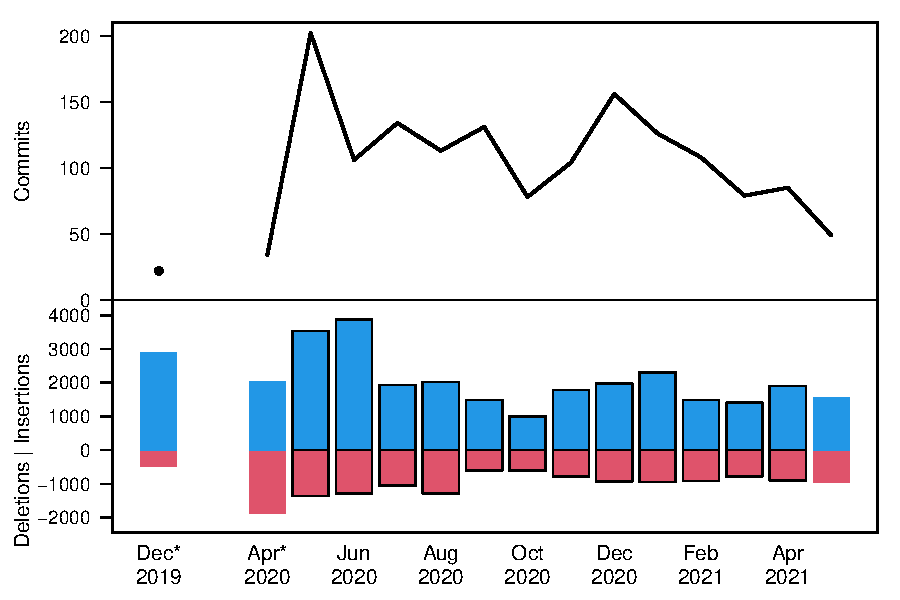
\includegraphics[width=0.57\textwidth]{svnplot_mon41}
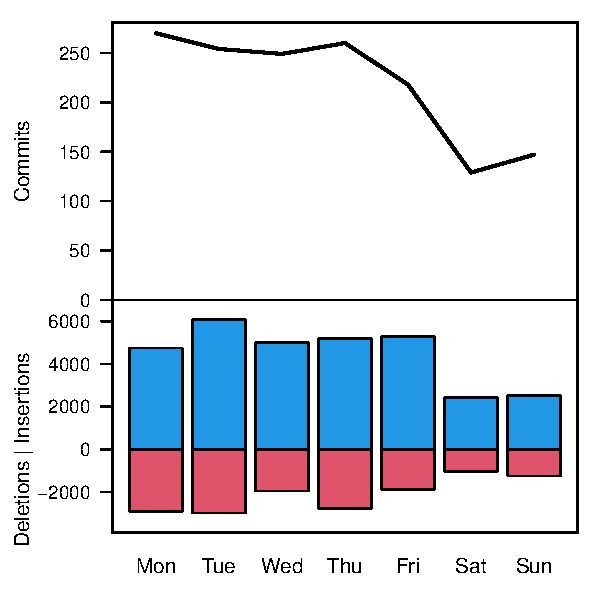
\includegraphics[width=0.38\textwidth]{svnplot_wd41}
\caption{Commit statistics by month (left) and weekday (right) during R 4.1.0 development.
*Note that the counts for April 2020 and May 2021 do not cover full months.
Commits from December 2019 represent work of Paul Murrell on the later
merged R-defs branch.}
\label{fig:svn41} \end{figure}

We observe an activity peak just after the release of R 4.0.0, a minimum in
October 2020, and otherwise relatively stable amounts of code changes.
The large numbers in May/June do not seem to follow a general
pattern: here Paul Murrell did most of his changes on graphics.
The right-hand plot shows that there is still a number of contributions even during the
weekends.

\section{R 4.1.0 bugs statistics}

Summaries of bug-related activities during the development of R 4.1.0 (from
April 25, 2020 to May 18, 2021) were derived from the database underlying
\href{https://bugs.R-project.org/bugzilla/}{R's Bugzilla system}. 
Figure~\ref{fig:bz41} shows statistics of reported/closed bugs and number of
added comments (on any bug report) by calendar month and weekday,
respectively.
Deviating from the previous issue, new bug reports (comment 0) are not
counted as comments, so these numbers cannot be compared directly.
Note that monthly statistics are impacted by truncation at the release
dates in April 2020 and May 2021, respectively.

Comments are added by reporters of the bugs, R Core members and external
volunteers.  When a bug report is closed, the bug is either fixed or the
report is found invalid.  In principle, this can happen multiple times for a
single report, but those cases are rare.  Hence the number of comments is a
measure of effort (yet a coarse one which does not distinguish thorough
analyses from one-liners) and the number of bug closures is a measure of
success in dealing with bugs.

R 4.1.0 was released by about 3 weeks later than usual, so the period which
is summarized is also longer.  The bug-related activities have still
increased much more than what could be explained by that: about 17\% more
bugs closed than for (during development of) 4.0.0, but 55\% more bugs
reported).  The increase from 3.6.0 to 4.0.0 was 45\% more bug reports and
92\% more bugs closed.

There was a significant increase in the number of comments following a
\href{https://developer.r-project.org/Blog/public/2019/10/09/r-can-use-your-help-reviewing-bug-reports}{blog
post} of Tomas Kalibera and Luke Tierney, published October 9, 2019 (so
during development of 4.0.0), asking the R community for help with the bugs. 
The rate of comments stayed relatively high until now, so for the
development of 4.1.0.  This increased activity also came with more bug
reports and more bugs closed.  Initially, more bugs were closed than
reported (4.0.0 development), but this changed during 4.1.0.  It may be that
the bugs fixed initially with the help of external volunteers were the older
ones easy to handle, but now there is space for external volunteers to help
with the new/harder ones.

\begin{figure}[htb]
\centering
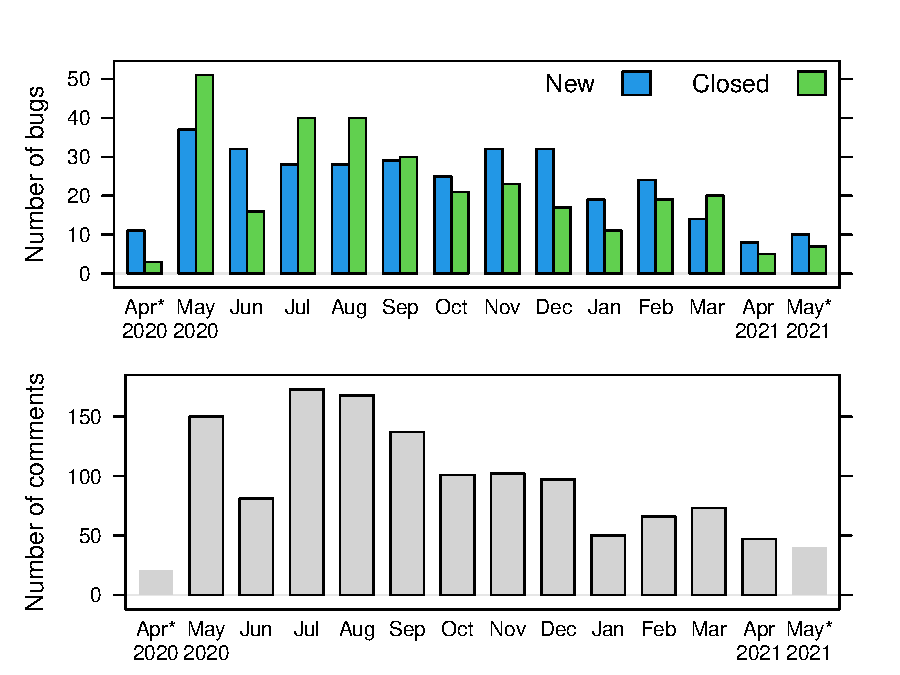
\includegraphics[width=0.57\textwidth]{apiplot_mon}
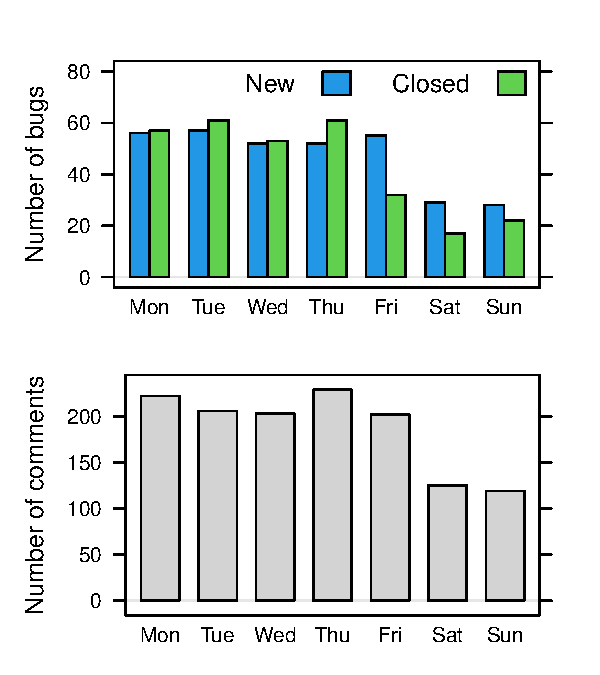
\includegraphics[width=0.38\textwidth]{apiplot_wd}
\caption{Bug tracking activity by month (left) and weekday (right) during R
4.1.0 development.  *Note that the counts for April 2020 and May 2021 do not
cover full months.
}
\label{fig:bz41}
\end{figure}

From the numbers by weekday in the right panel of Figure~\ref{fig:bz41} we
see that the R community still keeps working during the weekends.  Still,
the overall bigger bug-related activity seems relatively more reduced during
the weekends than during 4.0.0 and 3.6.0 development.


\section{Acknowledgements}
Tomas Kalibera's work on the article and R development has received funding
from the Czech Ministry of Education, Youth and Sports from the Czech
Operational Programme Research, Development, and Education, under grant
agreement No.CZ.02.1.01/0.0/0.0/15\_003/0000421, from the European Research
Council (ERC) under the European Union’s Horizon 2020 research and
innovation programme, under grant agreement No.  695412, and from the
National Science Foundation award 1925644.

\begin{samepage}
\address{Tomas Kalibera \\
  Czech Technical University, Czech Republic \\
  \email{Tomas.Kalibera@R-project.org}}

\address{Sebastian Meyer \\
  Friedrich-Alexander-Universit\"at Erlangen-N\"urnberg, Germany \\
  \email{seb.meyer@fau.de}}

\address{Kurt Hornik \\
  WU Wirtschaftsuniversit\"at Wien, Austria \\
  \email{Kurt.Hornik@R-project.org}}
\end{samepage}
